\chapter{虚拟专用网}
\question{什么是VPN}
VPN是一种依靠互联网服务提供商和其他网络服务提供商\textbf{在公共网络中建立专用的数据通信网络的技术}
\begin{itemize}
	\item 它是虚拟的网,即没有固定的物理连接,网络只有用户需要时才建立
	\item 他是利用公共网络设施构成的专用
\end{itemize}

\question{VPN的关键技术},通过各种技术满足通信安全,实现\textbf{身份认证、数据保密性、数据完整性}
\begin{enumerate}
	\item 隧道技术,将一种协议封装在另一种协议中传输,从而实现协议对公共网络的透明性
	\item 加密技术,隐藏传输信息的真实内容
	\item 密钥管理技术,确保在公网数据网上安全地传递密钥而不被窃取。
	\begin{enumerate}
		\item 手工配置,小网,更新不快
		\item 密钥交换歇息动态分发,适合复杂网,快速更新。需要PKI。
-	\end{enumerate}
	\item 用户认证技术
	\begin{enumerate}
		\item 仲裁认证
		\item 共享认证
	\end{enumerate}
\end{enumerate}

\question{隧道协议},根据协议所处的网络层次,可分为第二层隧道协议和第三层隧道协议。
\begin{enumerate}
	\item 第二层隧道协议,工作在数据链路层,吧龚总网络协议先封装到点对点协议中(PPP),然后进行隧道协议的封装,在通过数据链路层进行传输。
	\begin{enumerate}
		\item PPTP,点对点隧道协议。
		\item L2FP,第二层转发协议
		\item L2TP,第二层隧道协议
		\item MPLS,多协议标记交换
	\end{enumerate}
	\item 第三层隧道协议,工作在网络层
	\begin{enumerate}
		\item GRE,通用路由协议封装,主要规定如何用一种网络层协议去封装另一种网络层协议,不提供\textbf{加密功能},常与IPSec一起使用,由IPSec提供加密。
		\item IPSec,IP安全协议。可以对所有IP级的通信进行加密和认证。\
	\end{enumerate}
	\item 高层隧道协议
	\begin{enumerate}
		\item 安全套阶层SSL。位于TCP/IP与各种应用层协议之间,广泛地用于Web浏览器与服务器之间的身份认证和加密数据传输
		\begin{enumerate}
			\item SSL记录协议。它建立在可靠的传输协议(如TCP)之上,为高层提供\textbf{数据封装、压缩、加密}等基本功能的支持
			\item SLL握手协议。建立在SSL记录协议之上,用在实际的数据传输开始前,通信双方进行身份认证、协商加密算法、交换加密密钥等。
		\end{enumerate}
	\end{enumerate}
\end{enumerate}

\question{IPSec VPN}
IPSec VPN是IPSec的一种应用方式,其主要的应用场景可分为三种:
\begin{enumerate}
\item Site-to-Site(站点到站点或者网关到网关)。如一个机构的按个分之爱机构分布在互联网的3个不同地方,各使用一个网关相互简历VPN隧道,在机构内部网络之间的数据通过这些网关简历的IPSec隧道实现安全互联。
\item End-to-End(端到端或主机到主机):两个主机之间的通信由两台主机之间的IPSec绘画保护,而不是网关。
\item End-to-Site(端到站点或主机到网关):两台主机之间的通信由网关和异地户籍之间的IPSec进行保护
\end{enumerate}

\question{IPSec的设计目标}
\begin{enumerate}
\item 可认证IP报文的来源
\item 可保证IP报文的完整性
\item 可保护IP报文的私密性
\item 可防止认证报文被重放。
\end{enumerate}

\question{IPSec 的体系结构}
textbf{包括:}
\begin{enumerate}
	\item AH,验证头。为IP数据包提供无连接完整性与数据源认证,并提供保护以避免重播情况。\textbf{信息源的认证、信息的完整性防御、报文重发}
	\item ESP,封装安全载荷。加密需要保护的数据并且在IPSec ESP的数据部分进行数据的完整性校验,一次来保证机密性和完整性。\textbf{信息源的认证、
	信息的完整性、
	数据的私密性、
	防御报文重发}
	\item IKE,密钥管理协议,协商AH和ESP所使用的密码算法。
	\begin{enumerate}
	\item SA(安全联盟),描述通信对等体间对某些要素的约定,\textbf{单向的},实现双向通信,至少需要两个方向的数据流进行安全保护。\textbf{建立方式:}手工配置或者采用IKE自动协商方式。
	\item 和(ISAKMP)密钥管理协议。
	\end{enumerate}
	\item 用于验证和加密的一些算法
\end{enumerate}
IPSec工作时,首先两端的网络设备必须就SA达成一致。

\question{IPsec驱动程工作流程}
\begin{enumerate}
	\item 主机A向主机B发送一消息
	\item 主机A上IPsec驱动程序检查IP筛选器,查看数据包是否需要加密以及需要受到何种保护
	\item 驱动程序通知IKE开始安全协商
	\item 主机B上的IKE收到请求安全协商的通知
	\item 两台主机建立第一阶段SA对,各自共享主密钥
	\item 协商建立第二阶段SA对xxxx
\end{enumerate}
\textbf{P154}


\question{IPSec的工作模式}
\begin{enumerate}
	\item 隧道模式:封装了整个IP数据包,经过IPSec处理之后,在封装了一个外网IP头,主要用于Site-to-Site
	\begin{figure}[H]
		\centering
		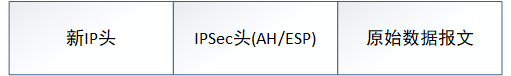
\includegraphics[width=0.7\linewidth]{figures/screenshot002}
		\caption{}
		\label{fig:screenshot002}
	\end{figure}
	
	\item 传输模式:仅仅封装IP数据包中上层协议信息,经过IPSec处理前后IP头部保持不变。主要用于End-to-End的应用场景。
	\begin{figure}
		\centering
		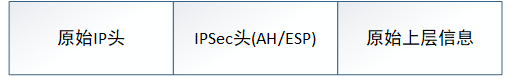
\includegraphics[width=0.7\linewidth]{figures/screenshot003}
		\caption{}
		\label{fig:screenshot003}
	\end{figure}
	
\end{enumerate}


\question{AH和ESP}
\begin{enumerate}
	\item AH 提供身份验证、完整性和防止重发,包含整个数据包的签名
	\begin{figure}[H]
		\centering
		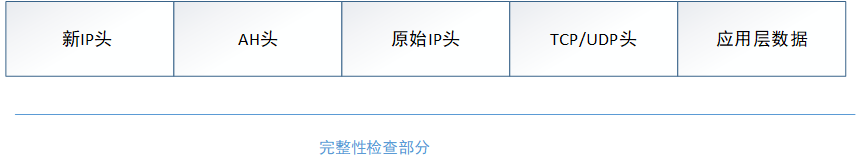
\includegraphics[width=0.7\linewidth]{figures/screenshot004}
		\caption{}
		\label{fig:screenshot004}
	\end{figure}
	\item ESP 除了AH的全部功能,还包括加密。通常不签署整个数据包,即通常只保护数据,而不保护IP头。ESP使用DES或者3DES加算法为数据包提供保密性。
	\begin{figure}[H]
		\centering
		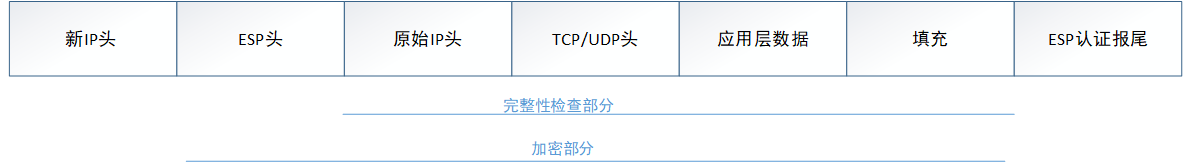
\includegraphics[width=0.8\linewidth]{figures/screenshot005}
		\caption{}
		\label{fig:screenshot005}
	\end{figure}
\end{enumerate}
 功能比较图:P155
 
 
 
\question{如何给一个信息系统定级}\\
信息系统定级需要考虑的两个重点:
\begin{enumerate}
	\item 受侵害客体
	\begin{itemize}
		\item 国家安全
		\item 社会秩序
		\item 个人安全
	\end{itemize}
	\item  受侵害的程度
	\begin{itemize}
		\item 一般影响
		\item 严重影响
		\item 特别严重影响
	\end{itemize}
\end{enumerate}
信息系统定级需要考虑的两个方面
\begin{enumerate}
	\item 信息安全:信息泄露、信息篡改
	\item 服务安全
\end{enumerate}

\question{等级保护的等级划分准则}
分为五级、级别越高危害程度越大。






















